\chapter[Resultados]{Experimentos e Resultados}
\label{resultados}
Nessa seção, detalhes dos experimentos realizados, bem como os resultados experimentais são mostrados a partir de simulações utilizando as bases de dados apresentadas na \secref{metodologia}.

\section{Análise \textit{dataset DataMining}}  
Na \figref{fig:ResultsMining} têm-se os gráficos de taxa de acerto em função dos diferentes limiares simulados para o \textit{dataset} proposto por \cite{DataMining}. Para valores de limiar entre 0.8 e 0.84 a taxa de acerto permanece acima de 98.4\% e conforme o aumento do limiar, a taxa de acerto vai decrescendo. Tal comportamento é esperado, visto que para valores altos de limiar, o tráfego analisado deve ter propriedades (entropia, variação de IPs origem e taxa de pacotes) muito próximas do perfil normal para não ser considerado um ataque. Desta forma, vale ressaltar que existem diferentes tipos de ataques DDoS, os quais geralmente possuem abordagens singulares para a realização dos mesmos. Dessa forma, a escolha de limiares próximos a um não representam uma boa escolha para este tipo de problema, uma vez que a granularidade dos ataques não seria abrangida pelo \textit{framework}. Na tabela \tabref{Tab:ResultsMining} são mostrados  o número de acertos, falsos positivos e falsos negativos na análise do \textit{dataset}, complementando o gráfico apresentando na \figref{fig:ResultsMining}.

 \begin{figure}[htb]
 	\centering
 	\caption{Análise do \textit{dataset} avaliado }
 	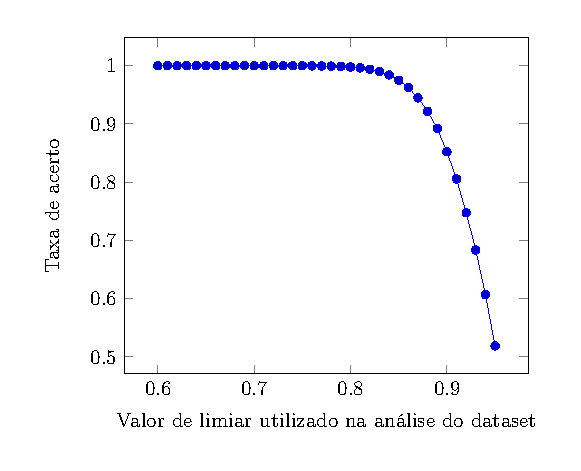
\includegraphics[width=0.9\textwidth]{figs/results80-95Mining.pdf}\\
 	\hspace{1.5cm}{Fonte: Elaborada pelo autor.}
 	\label{fig:ResultsMining}
 \end{figure}
 
 \begin{table}[htb]
 	\centering
 	\begin{threeparttable}
 		\caption{Exemplo base de dados Data Mining}
 		\label{Tab:ResultsMining}
 		%	\small
 		\begin{tabular}{c c c c}
 			\toprule
 			\textbf{Limiar} & \textbf{Taxa de acerto} & \textbf{Taxa de falsos positivos} & \textbf{Taxa de falsos negativos}
 			\\ \midrule
	 			
 			0.60 &  100\% &  0\%& 0\%   \\ \midrule
 			0.62 &  99.9996\% &  0\%& 0.0003996\%   \\ \midrule
 			0.64 &  99.9996\% &  0\%& 0.0003996\%   \\ \midrule
 			0.66 &  99.9996\% &  0\%& 0.0003996\%   \\ \midrule
 			0.68 &  99.9996\% &  0\%& 0.0003996\%   \\ \midrule
 			0.70 &  99.9992\% &  0\%& 0.0007993\%   \\ \midrule
 			0.72 &  99.9992\% &  0\%& 0.0007993\%   \\ \midrule
 			0.74 &  99.9992\% &  0\%& 0.0007993\%   \\ \midrule
 			0.76 &  99.9800\% &  0\%& 0.0.01998\%   \\ \midrule
 			0.78 &  99.9664\% &  0\%& 0.03357\%   \\\midrule 		 			 			 			 			 			 			 			
 			0.80 &  99.7790\% &  0\%& 0.2210\%   \\ \midrule
 			0.82 &  99.3905\% & 0\% & 0.6095 \%   \\ \midrule
 			0.84 &  98.4137\%  & 0\% & 1.5863\%   \\ \midrule
 			0.86 &  96.2556\%  &  0\% & 3.7444\%   \\ \midrule
 			0.88 &  92.1842\%  &  0\% & 7.8158\%     \\ \midrule
 			0.90 &  85.2309\%  & 0\% & 14.7691\%    \\ \midrule
 			0.92 &  74.7722\%  &  0\% & 25.2278\%   \\ \midrule
 			0.94 &  60.6753\%  & 0\% & 39.3247\%   \\ \bottomrule
 		\end{tabular}
 		{Fonte: Elaborada pelo autor.}
 	\end{threeparttable}
 \end{table}
Como pode ser visto na tabela \tabref{Tab:ResultsMining}, a coluna "Taxa de falsos positivos" não apresentou nenhuma ocorrência (0\%). Esse fato, deve-se especialmente a natureza do \textit{dataset} ser apenas de ataques e, dessa forma possuir uma correlação mais forte em comparação com a de um tráfego normal. Já na coluna "Taxa de falsos negativos" (tráfego de ataque que foi considerado normal) apresentou, dependendo do valor de limiar, um número considerável de eventos.
\section{Análise \textit{dataset} DARPA}
Outra base de dados avaliada pelo \textit{framework} é o DARPA conforme descrito na \secref{metodologia}.
A \figref{fig:ResultsDarpa} apresenta os gráficos das taxas de acertos em função dos limiares simulados. Para limiares entre 0.64 e 0.68, as taxas de acertos ficam entre 60 a 85\%. Tal comportamento é diferente da base de dados anterior, pois tratam-se de bases que diferem em termos de tratamento temporal, modo de detecção e arquivo de respostas, já que no DARPA é mostrada uma janela de tempo onde provavelmente o ataque nomeado irá ocorrer, enquanto no \textit{Datamining} tem-se uma base constituída apenas por ataques. Além disso, conforme explanado na \secref{metodologia}, o \textit{framework} teve que ser adaptado para analisar o \textit{dataset}, sendo possível analisar a base a qual contém apenas ataques. Logo, espera-se que os valores sejam diferentes para ambos os \textit{datasets}. A \tabref{Tab:ResultsDARPA} mostra as taxas de acertos, falsos positivos e falsos negativos resultantes da análise. O \textit{framework} possui baixa taxa de falsos negativos, tendo em vista que a taxa de detecção é máxima para a maioria dos limiares simulados, mostrando a eficiência do método de detecção.       
 \begin{figure}[htb]
 	\centering
 	\caption{Análise do \textit{dataset} avaliado }
 	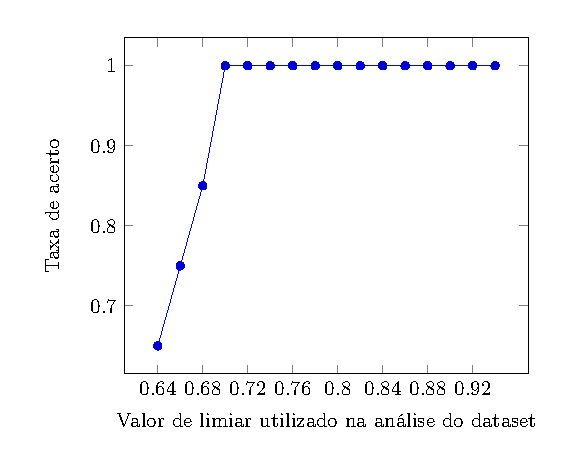
\includegraphics[width=0.85\textwidth]{figs/resultsDarpa.pdf}\\
 	\hspace{1.5cm}{Fonte: Elaborada pelo autor.}
 	\label{fig:ResultsDarpa}
 \end{figure}
 
  \begin{table}[htb]
  	\centering
  	\begin{threeparttable}
  		\caption{Exemplo base de dados DARPA}
  		\label{Tab:ResultsDARPA}
  		%	\small
  		\begin{tabular}{c c c c}
  			\toprule
  			\textbf{Limiar} & \textbf{Taxa de acerto} & \textbf{Taxa de falsos positivos} & \textbf{Taxa de falsos negativos}
  			\\ \midrule
  			0.64 &  65\% &  0\%& 35\%   \\ \midrule
  			0.66 &  75\% & 0\% & 25 \%   \\ \midrule
  			0.68 &  85\%  & 0\% & 15\%   \\ \midrule
  			0.70 &  100\%  &  0\% & 0\%   \\ \midrule
  			0.72 &  100\%  &  0\% & 0\%     \\ \midrule
  			0.74 &  100\%  & 0\% & 0\%    \\ \midrule
  			0.76 &  100\%  &  0\% & 0\%   \\ \midrule
  			0.78 &  100\%  &  0\% & 0\%   \\ \midrule
  			0.80 &  100\%  &  0\% & 0\%   \\ \midrule
  			0.82 &  100\%  &  0\% & 0\%   \\ \midrule
  			0.84 &  100\%  &  0\% & 0\%   \\ \midrule
  			0.86 &  100\%  &  0\% & 0\%   \\ \midrule
  			0.88 &  100\%  &  0\% & 0\%   \\ \midrule
  			0.90 &  100\%  &  0\% & 0\%   \\ \midrule
  			0.92 &  100\%  &  0\% & 0\%   \\ \midrule
   			0.94 &  100\%  & 0\% & 0\%   \\ \bottomrule
  		\end{tabular}
  		{Fonte: Elaborada pelo autor.}
  	\end{threeparttable}
  \end{table}

A \figref{fig:ResultsNHOQUE} mostra os resultados obtidos por \cite{HOQUE201748} para a análise do \textit{dataset} DARPA. Vale ressaltar que na referência, a versão exata do \textit{dataset} não foi explicitada. No entanto, os gráficos possuem semelhança em seus valores de taxa de acerto, sendo possível considerar validado o \textit{framework}.  
 \begin{figure}[htb]
 	\centering
 	\caption{Resultados artigo \cite{HOQUE201748} }
 	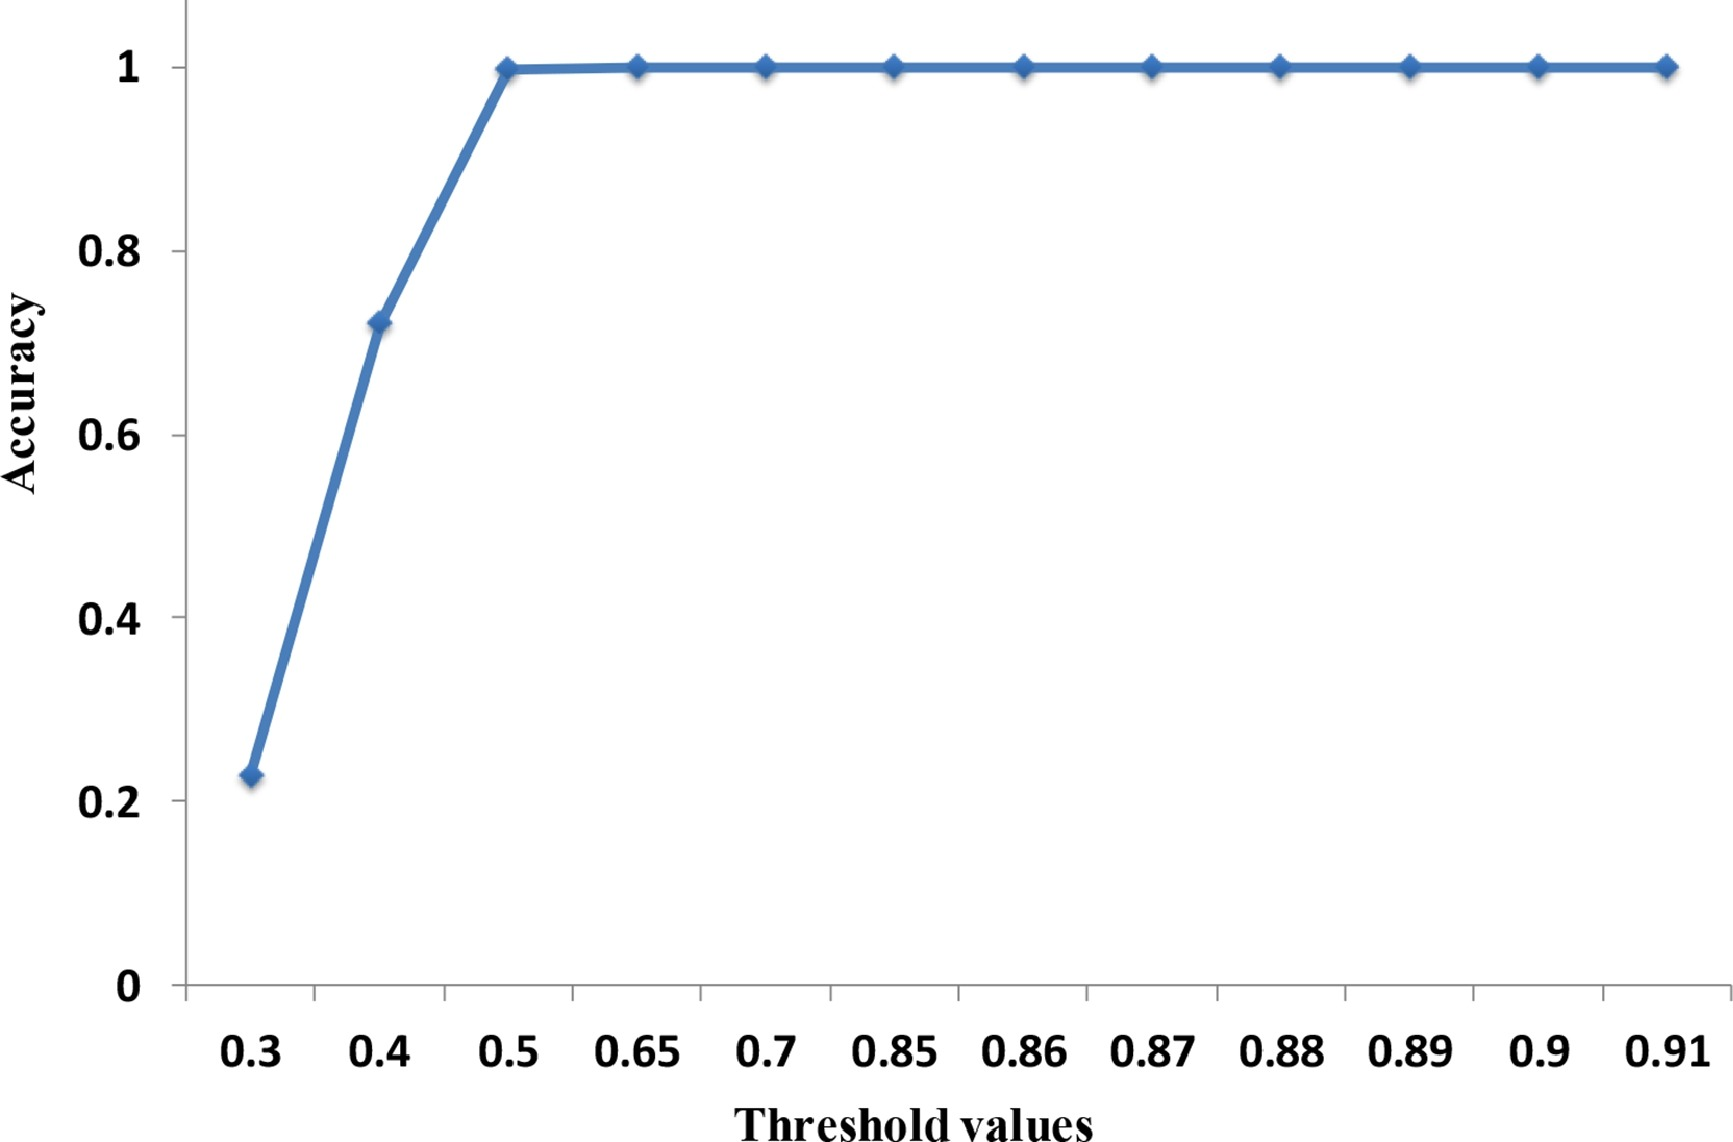
\includegraphics[width=0.7\textwidth]{figs/resultNHOQUE.jpg}\\
 	\hspace{1.5cm}{Fonte: \cite{HOQUE201748}.}
 	\label{fig:ResultsNHOQUE}
 \end{figure}

   Para limiares acima de 70\%, ambos os gráficos têm 100\% de acerto. Assim, ao escolher um intervalo válido de limiares para realizar a detecção deve-se levar em conta os valores para os quais a detecção teve maiores taxas de acerto.